
\section{Wat is een PWA}
\label{ch: Wat is een PWA}


Het web is een platform waar applicaties kunnen gepubliceerd worden zonder afhankelijk te zijn van een overkoepelend bedrijf of organisatie. Voor een website is er slechts één codebase en de laatste versie is steeds beschikbaar voor de gebruiker. 
Dit allemaal zorgt ervoor dat een webapplicatie iedereen overal kan bereiken en dit op elk mogelijk toestel.

Native applicaties zijn betrouwbaar en bieden een heel goede gebruikerservaring. Ze starten op als een alleenstaande toepassing en ze kunnen uitgebreid gebruik maken van het besturingssysteem: ze kunnen bestanden lezen en schrijven, gebruik maken van usb-connecties en bluetooth, ze hebben toegang tot de contacten en de kalender en nog veel meer. Native applicaties voelen aan alsof ze deel uitmaken van het toestel waarop ze werken.

We kunnen dus stellen dat webapplicaties de bovenhand hebben in bereik maar dat native applicaties de bovenhand hebben als het op functies aankomt.

Een Progressive web application (PWA) is een webapplicatie die gebruik maakt van moderne web API’s om functies aan te bieden die voordien enkel beschikbaar waren voor native applicaties. De bedoeling van ' is om de sterktes van webapplicaties (het bereik) en native applicaties (de functionaliteit) te combineren. 
\autocite{Richard2020}
\autocite{Google2020}

Voorbeelden van deze extra functionaliteiten die PWA's kunnen hebben zijn: 

\begin{itemize}
	\item Een PWA kan toegevoegd worden aan het startscherm van een toestel.
	\item Een PWA kan push notificaties ontvangen.
	\item Een PWA kan offline ook gebruik worden.
\end{itemize}




\begin{figure}[!htb]
	\centering
	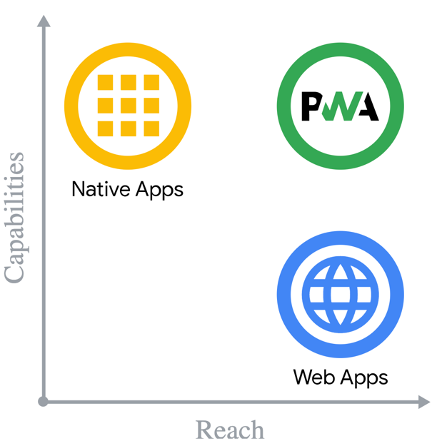
\includegraphics{./img/WatIsEenPwa.png}
	\caption{voorstelling van wat is een PWA \autocite{Richard2020}}
\end{figure}


\subsection{Service workers}

	De service worker is een script dat veel functionaliteiten beschikbaar maakt die voordien enkel beschikbaar waren voor native applicaties. In dit hoofdstuk wordt er bekeken welke functionaliteiten de service worker juist beschikbaar maakt voor een PWA en hoe dit gebeurt. 
	
	
	
	\subsubsection{Wat is een service worker}
	\label{ch: Wat is een servcie worker}
	
		Een service worker is een web worker die tussen het netwerk en de applicatie wordt geplaatst. Dit zorgt ervoor dat de service worker inkomende en uitgaande netwerkverzoeken kan controleren en eventueel manipuleren.
		\autocite{Mozilla2020}
		
		Een web worker is een script dat in de achtergrond van een applicatie werkt en die onafhankelijk is van de andere scripts. Web workers hebben dus geen impact op de prestaties van de webapplicatie die er gebruik van maakt.  Web workers hebben geen toegang tot het Document Object Model (DOM) van een webapplicatie, ze kunnen de inhoud van een website dus niet rechtstreeks manipuleren.
		\autocite{Verdu2015}
		\autocite{Hiltunen2018}
		
		
		Services workers werken dus constant op de achtergrond, maar de manier waarop service workers opgebouwd zijn (
	zie hoofdstuk \ref{ch: Wat is een servcie worker}) heeft geen significante invloed op de batterijduur van een mobiel toestel.
		\autocite{Malavolta2016}
	
	
	\subsubsection{Functionaliteiten die een serivce worker mogelijk maakt}
	\label{ch: Functionaliteiten die een serivce worker mogelijk maakt}
	
		De service worker werkt onafhankelijk van de applicatie. Dit houdt in dat een service worker wel nog kan werken terwijl de applicatie afgesloten is. Hierdoor zijn volgende functies mogelijk binnen een webapplicatie:
	
		
		
		\paragraph{Offline gebruik}
		
			Als een PWA voor een eerste keer geladen wordt op een toestel zullen de bezochte pagina's offline beschikbaar blijven. Dit gebeurt door de  HTML, CSS en JavaScript bestanden die nodig zijn om de pagina's te creëren lokaal op te slaan. Applicaties die geen gebruik maken van netwerkverzoeken om data te laden, zullen dus offline volledig werken.
			
			Met service workers kunnen netwerkverzoeken en pagina’s ook gecached worden. Als een pagina geladen wordt, kunnen alle elementen opgeslagen worden op het toestel. Als deze pagina later opnieuw bezocht wordt, hoeft deze niet meer aan de server gevraagd te worden. Hierdoor wordt de applicatie sneller en minder afhankelijk van de netwerkverbinding.
			Volgens onderzoek, dat uitgevoerd werd door Google, verlaten 53\% procent van de gebruikers een website als deze niet geladen is binnen 3 seconden. Service workers kunnen dus helpen om het aantal gebruikers op jouw website te verhogen.
			\autocite{Google2017}
			
			De twee mechanismes die gebruikt worden om data offline beschikbaar te maken zijn ‘indexedDB’ en de ‘cache API’.
			\autocite{Osmani2019}
			\autocite{Mozilla2020a}
			
			
			

			\subparagraph{Cache API}

				De cache API wordt gebruikt om data die verkregen werd van netwerkverzoeken op te slaan. Zowel de ‘request’ als de ‘response’ van een netwerkverzoek kunnen in de cache API opgeslagen worden.
				\autocite{Scales2019}

			\subparagraph{IndexedDB}

				IndexedDB is een mechanisme dat gebruikt wordt om lokaal gestructureerde data op te slaan. Het kan vergeleken worden met object georienteerde databasemanagementsystemen die gebruik maken van JavaScript objecten om data op te slaan. Een IndexedDb maakt gebruik van indexen. Dit heeft als voordeel dat het uitlezen van data snel kan gebeuren
				\autocite{Mozilla2019}
	
	
	\paragraph{Notificaties}
	
		Er zijn twee soorten notificaties: lokale notificaties en push notificaties. 
		Lokale notificaties worden geactiveerd vanop de applicatie van de gebruiker, er zijn geen externe invloeden die deze notificatie activeren.
		
		Binnen lokale notificaties kunnen we nog het onderscheid maken tussen persistente en niet-persistente notificaties.
		Niet-persistente notificaties zijn notificaties die enkel getoond kunnen worden als de applicatie geopend is. Dit type notificaties heeft geen service worker nodig. 
		Persistente notificaties zijn notificaties die nog steeds geactiveerd worden vanuit de code op het toestel, maar de applicatie moet niet meer actief zijn. Hier is wel een service worker nodig.
		{\tiny }
		Push notificaties worden niet geactiveerd binnen de applicatie, maar worden geactiveerd door een server.
		Om push notificaties te gebruiken, moet er gebruik gemaakt worden van twee webAPI’s: de notifications API en de Push API.
		
		\subparagraph{Notifications API}
			Dit is een API die het uiterlijk en het gedrag van een notificatie zal bepalen. Deze API wordt zowel gebruikt voor lokale als voor push notifications.
			Om gebruik te maken van deze API moet de gebruiker expliciet toegang geven aan de applicatie.
			
			Een voorbeeld van de code van een notificatie kan er als volgend uitzien
		
	
		
\begin{lstlisting}
function displayNotification() {
  if (Notification.permission == 'granted') {
   navigator.serviceWorker.getRegistration().then(function(reg) {
     var options = {
       body: 'Here is a notification body!',
       icon: 'images/example.png',
       vibrate: [100, 50, 100],
       data: {
         userId: “383209489398274”
       },
       actions: [
         {action: 'explore', title: 'Explore this new world',
           icon: 'images/checkmark.png'},
         {action: 'close', title: 'Close notification',
           icon: 'images/xmark.png'},
       ]
     };
     reg.showNotification('Hello world!', options);
   });
  }
}
\end{lstlisting}
		

		
			Om een notificatie weer te geven, wordt er een object verwacht waar de inhoud van de melding wordt vastgelegd. Volgende keys kunnen meegegeven worden:
			
				
			\begin{table}[H]
				\centering
				\begin{tabular}{cp{12cm}}
			       body & De boodschap die in de melding staat  \\
			       icon & Het icoontje dat in de notificatie wordt getoond. \\
			       vibrate & Het vibratiepatroon dat de melding zal maken in milliseconden. \\
			       data & Data is een object dat gebruikt kan worden als de gebruiker op de notificatie  klikt. Dit object zal dan ontvangen worden in de applicatie. Hier zal vaak het id van de gebruiker teruggevonden worden. \\
			       actions & Er kunnen ook acties toegevoegd worden aan de melding. Elk object in deze array zal een knop worden op de melding met een andere functie. Het gedrag van de knoppen wordt bepaald in de applicatie aan de hand van de ‘action’. \\
				\end{tabular}	
				\caption{beschrijving Notifications API}
			\end{table}
			\autocite{Developers2019}
			\autocite{Mozilla2019a}
		
		
		
		\subparagraph{Push API}
		
			De push API wordt gebruikt door de service worker. Als de server een notificatie verstuurt, wordt deze opgevangen door de push API. Deze API zal dan gebruik maken van de notifications API om een melding op het toestel van de eindgebruiker te tonen.
			\autocite{Mozilla2019b}
			\autocite{Gaunt2020}
	
	\paragraph{Achtergrondsynchronisatie }
		Een PWA kan gebruik maken van de background sync API om achtergrondsynchronisatie toe te passen.
		
		Achtergrondsynchronisatie kan toegepast worden als er een trage of geen netwerkverbinding is. 
		
		Achtergrondsynchronisatie is het proces waarbij een netwerkverzoek, dat uitgevoerd werd als er geen of een te zwakke internetverbinding was, wordt opgeslagen in de service worker en wordt uitgevoerd als er wel een stabiele internetconnectie is.
		
		Een voorbeeld hiervan is het verzenden van een bericht via een sociaal media platform. Als het bericht verzonden wordt terwijl de gebruiker offline is, zal er geen fout getoond worden maar zal dit bericht verzonden worden vanaf er internet is.
		
		Google Chrome op Android maakt hier gebruik van. Als er een website bezocht wordt als er geen internetverbinding is, krijgt de gebruiker de melding: “Chrome laat je weten wanneer de pagina klaar is”. Vanaf het toestel terug een internetverbinding heeft, en het de pagina heeft kunnen downloaden,  zal de gebruiker een melding krijgen die met de boodschap dat de pagina bekeken kan worden.
	
	
		\begin{figure}[H]
			\centering
			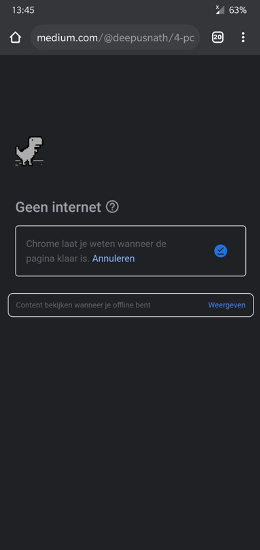
\includegraphics[width=35mm]{./img/backSync1.png}{}
			\caption{demonstratie van achtergrond synchrondisatie bij Google Chrome op Android - pagina offline}
		\end{figure}
		
		\begin{figure}[H]
			\centering
			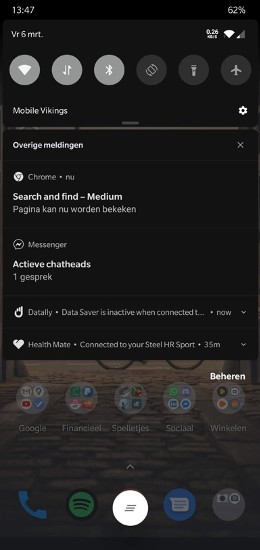
\includegraphics[width=35mm]{./img/backSync2.png}
			\caption{demonstratie van achtergrond synchrondisatie bij Google Chrome op Android - melding als gebruiker terug online is}
		\end{figure}
		 
	
	
		\subsubsection{Service worker lifecycle }
		De levenscyclus van de service worker is onafhankelijk van de levenscyclus van de webapplicatie. Als de webapplicatie gesloten wordt, blijft de service worker gewoon werken.
		
		Om een service worker te installeren moet deze geregistreerd worden in de javascript van de webapplicatie. Dit gebeurt normaal bij het eerst bezoek aan de website van de gebruiker.
		
\begin{lstlisting}
function displayNotification() {
if ('serviceWorker' in navigator) {
	navigator.serviceWorker.register('/service-worker.js');
}
\end{lstlisting}
	
		Als een service worker wordt geïnstalleerd, worden de opgegeven statische bestanden (foto’s, css-bestanden, javascript-bestanden) gedownload. Als dit slaagt, wordt er naar de activatiefase gegaan, als dit niet slaagt zal dit proces zich herhalen tot het slaagt. 
		
		Tijdens de activatiefase wordt er bekeken welke gecachete gegevens geüpdatet moeten worden en welke niet. De service worker zal de bestanden die het ontvangen heeft van het eerste netwerkverzoek vergelijken met zijn huidig cachegeheugen. Als er verschillen zijn zal dit cachegeheugen aangepast worden.
		
		ls de activatiefase geslaagd is, heeft de service worker controle over de pagina’s die binnen zijn scope vallen. Deze scope moet gedefinieerd worden binnen de service worker.
		
		Nu het oude cachegeheugen up-to-date is, zal de service worker overgaan naar een “rust”-toestand, hierbij wacht de service worker op netwerkverzoeken van bestanden die binnen zijn scope vallen.
		
		Als er een netwerkverzoek wordt verstuurd, zal de service worker deze verzoeken afhandelen. Na een bepaalde tijd zal de service worker terug naar de ‘rust’-modus gaan tot er een nieuw netwerkverzoek is. De service worker gaat naar deze ‘rust’-toestand om zowel cpu-kracht als geheugen te sparen.
		\autocite{Gaunt2019}
		
		
		\begin{figure}[H]
			\centering
			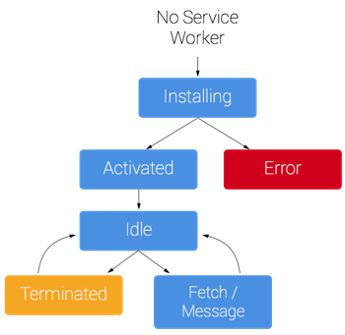
\includegraphics{./img/ServiceWorkerLifeCycle.png}
			\caption{schema levenscyclus van een service worker \autocite{Gaunt2019}}
		\end{figure}
	

\subsection{A2HS}
	
	Als een applicatie voldoet aan bepaalde criteria, kan deze geïnstalleerd worden op het toestel van de gebruiker. Deze functie is beschikbaar voor verschillende besturingssystemen: Windows, Mac OS, Android, IOS.
	
	Een website moet voldoen aan volgende criteria:
	
	\begin{itemize}
		\item	Nog niet geïnstalleerd zijn
		\item	Een HTTPS-connectie hebben
		\item	Een manifest.json bestand hebben
		\item	Een service worker registreren.
	\end{itemize}
	
	Als een website aan alle criteria voldoet zal er een beforeinstallprompt event gestart worden. Elke browser gaat hier anders mee om. 
	
	\begin{figure}[H]
		\centering
		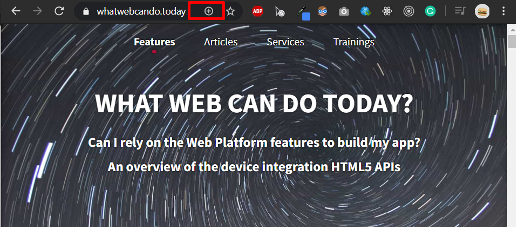
\includegraphics{./img/beforeinstallprompt_windows.png}	
		\caption{gedrag van Google Chrome op Windows 10 op het beforeinstallprompt}
	\end{figure}
	
	\begin{figure}[H]
		\centering
		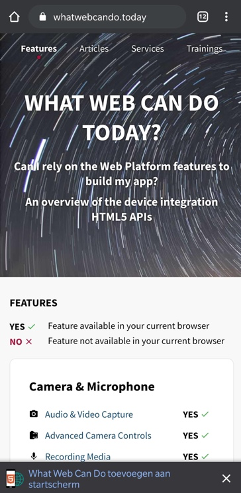
\includegraphics{./img/beforeinstallprompt_android.png}
		\caption{gedrag van Google Chrome op Android op het beforeinstallprompt}
	\end{figure}
	
	Op Apple toestellen (IPhone, Mac) heeft het beforeinstallprompt geen effect. De gebruiker moet zelf op zoek gaan in het menu om de applicatie te installeren, maar dit is wel mogelijk.
	
	Het beforeinstallprompt kan wel in de code opgevangen worden. De  gebruiker kan dan geïnformeerd worden dat deze webapplicatie geïnstalleerd kan worden. 
	Niet alle gebruikers zullen weten hoe ze dit moeten doen, het is dus aangeraden om de gebruiker hierin te begeleiden door hem duidelijke instructies te geven.
	\autocite{PWAbuilder2020}


\subsection{Application shell}
	De application shell of app shell is de minimale HTML, CSS en JavaScript die nodig is om een userinterface te tonen op een toestel. Dit is vaak de header, footer en de navigatie.
	
	Door de bestanden die steeds terugkomen offline op te slaan, worden deze veelgebruikte elementen onmiddellijk geladen. Dit zorgt ervoor dat een webapplicatie meer zal aanvoelen als een native applicatie.
	
	Het toepassen van deze architectuur biedt een aantal voordelen:
	
	\begin{itemize}
		\item	Consistent snel
		\item	Voelt native aan
		\item	De gebruiker moet minder data downloaden
	\end{itemize}
	\autocite{Osmani2019a}
	
	\begin{figure}[!htb]
		\centering
		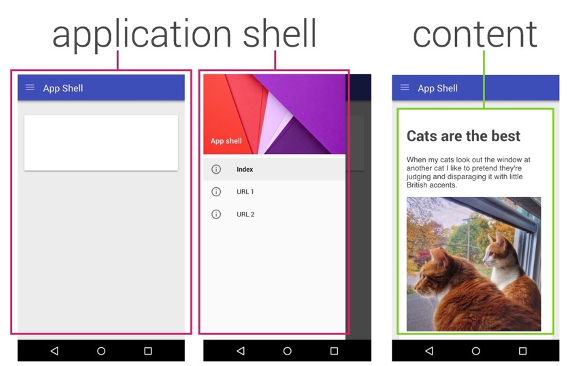
\includegraphics{./img/ApplicationShell.png}
		\caption{voorbeeld van een application shell architectuur \autocite{Osmani2015}}
	\end{figure}
	

\subsection{Progressive enhancement}
	Progressive enhancement is een strategie bij webontwikkeling waarbij er gezorgd wordt dat alle hoofdfunctionaliteiten beschikbaar zijn op alle toestellen. Meer geavanceerde functies worden aan deze basisversie toegevoegd. 
	
	Het doel van progressive enhancement is dat een applicatie gebruikt kan worden op elk toestel en dat meer modernere toestellen of browsers van een rijkere ervaring kunnen genieten.
	\autocite{Vanhala2017}
	
	
\subsection{Application manifest}
	Het web app manifest is een JSON-bestand dat informatie bevat over de applicatie. Deze informatie is nodig voor het installeren van een PWA op een toestel.
	Aan de hand van dit bestand weet het besturingssysteem bijvoorbeeld welk icoon er gebruikt moet worden en hoe het startscherm er moet uitzien.
	
	Voorbeeld van een minimum app manifest voor de Google Maps PWA.
	
\begin{lstlisting}
{
"short_name": "Maps",
"name": "Google Maps",
"icons": [
 {
   "src": "/images/icons-192.png",
   "type": "image/png",
   "sizes": "192x192"
 },
 {
   "src": "/images/icons-512.png",
   "type": "image/png",
   "sizes": "512x512"
 }
],
"start_url": "/maps/?source=pwa",
"background_color": "#3367D6",
"display": "standalone",
"scope": "/maps/",
"theme_color": "#3367D6"
}
\end{lstlisting}
	
	
		\begin{table}[H]
			\centering
			\begin{tabular}{cp{12cm}}
	     		short\_name & Naam van de applicatie die op het startscherm gebruikt zal worden. Deze mag maximaal 12 karakters lang zijn. \\
	     		name & Naam die op alle andere plekken gebruikt zal worden: vb bij de vraag als de app geïnstalleerd mag worden. Deze mag maximaal 45 karakters lang zijn. \\
	     		icons & Een lijst vna objecten die het icoon bepaalt dat de applicatie zal gebruiken.
Verschillende platformen vragen verschillende type's iconen Dit object heeft volgende eigenschappen:
		     		\begin{itemize}
			    		  \item src - bron van het icoont
			    		  \item type - het bestandstype van het icoon
			    		  \item size - de afmeting van het icoon
	     			\end{itemize} \\
	     		start\_url & De url naar waar de PWA moet gaan als de applicatie gestart wordt vanaf het startscherm van een toestel.\\
	     		background\_color & Hier wordt een kleur gedefinieerd. Dit kleur zal gebruikt worden voor het opstartscherm. \\
	     		display & Dit bepaalt in wat voor webview de PWA getoond zal worden. Mogelijkheden zijn:
		     		\begin{itemize}
			     		  \item fullscreen – opent de browser zonder UI-elementen (adresbalk, terug knop, ….)
			     		  \item standalone – opent de applicatie als een native applicatie los van de browser. Er worden geen UI-elementen van de browser getoond.
			     		  \item nimal-ui – opent de applicatie in de browser maar toont slechts beperkte UI elementen van de browser. De adresbalk is weg maar de ‘vorige’ knop is er nog.
			     		  \item browser – opent de PWA in een normaal browser tabblad.
		     		\end{itemize} \\
	     		scope & De scope bepaalt alle links die binnen de PWA vallen. \\
	     		theme\_color & De kleur die de adresbalk zal innemen.
			\end{tabular}	
			\caption{beschrijving minimum application manifest}
		\end{table}
				
			
	
	
	\autocite{LePage2020}

\subsection{Geschiedenis van PWA's}

	\subsubsection{"One last thing"}
	
		 “One last thing” is de zin waarmee Steve jobs, co-founder van Apple, zijn jaarlijkse toespraak steeds afsloot. Er volgde meestal een revolutionair idee of product dat Apple zal uitbrengen.
		
		In juni 2007 sloot Steve Jobs, nadat hij net de eerst IPhone had voorgesteld, zijn toespraak af met de visie die Apple toen had over hoe het web er moet uitzien. De term progressive web apps bestond nog niet, maar de concepten die hij uitlegde zijn wel de basis van '. Steve Jobs citeerde volgende stellingen
	
		
		\begin{itemize}
			\item \textit{ “We have got an inovative way to create applications for mobile devices, and it’s all based on the fact that IPhone has the full Safari engine on board”}
			\item \textit{ “You can write apps that look like IPhone apps and that integrate with IPhone services”}
			\item \textit{ “Instant distribution, just put them on the internet”}
			\item \textit{ “They are really easy to update, just put the update on your server”}
		\end{itemize}
		\autocite{Jobs2007}
		
		Apple had verwacht dat dit een succes zou zijn. Maar de ontwikkelaars waren teleurgesteld en ze hadden verwacht dat ze meer toegang zouden krijgen tot de IPhone. In de eerste versie van de IPhone kon enkel gebruik gemaakt worden van de apps die geïnstalleerd waren door Apple, er konden geen nieuwe apps gedownload worden.
		\autocite{Strieb2016}
		
		 De visie van Apple veranderde echter toen ze het volgend jaar de app-store lanceerden. \autocite{Silver2018}
	 
	 \subsubsection{Crome dev summit 2015}
	 
		 Chrome dev summit is een conferentie voor webontwikkelaars georganiseerd door Google. 
		 
		 Alex Russel en Andreas Bovens gebruikten voor het eerst de term “progressive web apps”. Op dit moment ondersteunde enkel Android service workers en A2HS.
		 
		 Ook werd het concept van de application shell voorgesteld.
		 \autocite{Russel2015}
	 
	 
	 \subsubsection{IOS 13}
		 Op 19 september 2019 stelde Apple IOS 13 voor. Deze software-update zorgde ervoor dat de IPhone gebruik kon maken van een service worker. De applicaties kunnen nu ook geïnstalleerd worden op het toestel, de gebruiker moet dit wel nog zelf doen aan de hand van het menu.
		 \autocite{Apple2020}
	 


\subsection{Voorbeelden van PWA's}
	
	\subsubsection{Outlook}
		Google is niet de enige grote speler die ' wil promoten en implementeren.
		\autocite{Microsoft2020}
		
		Microsoft geeft het goede voorbeeld door de veelgebruikte email client Outlook ook beschikbaar te maken als een PWA.
		De PWA-versie van de applicatie is slechts 800KB groot terwijl de traditionele versie op een desktop 1,8GB groot is.
		\begin{figure}[H]
			\centering
			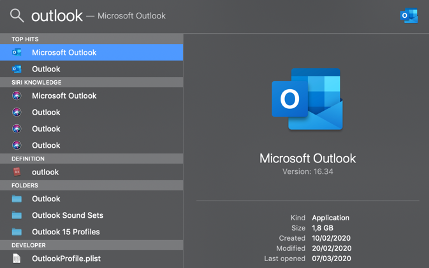
\includegraphics{./img/Outlook_native.png}
			\caption{Outlook op Mac}
		\end{figure}
		
		\begin{figure}[H]
			\centering
			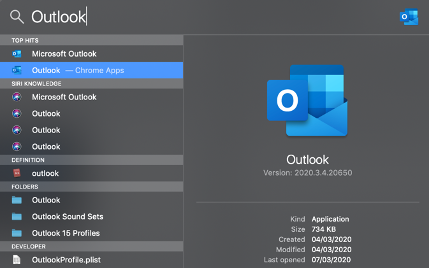
\includegraphics{./img/Outlook_pwa.png}
			\caption{Outlook op Mac als PWA}
		\end{figure}
		
	
	
	
	
	\subsubsection{AliExpress}
		
		AliExpress, één van de grootste e-commerce platformen, implementeerde hun website als een PWA. De resultaten waren heel positief, bij nieuwe gebruikers werd er 104\% meer verkocht. De gemiddelde gebruiker bleef ook 74\% langer op de website.
		\autocite{Developers2020}
	
	
	\subsubsection{Twitter}
	
		Twitter, één van de grootste sociale media platformen, implementeerde hun website ook als PWA. De resultaten waren ook hier positief. Het datagebruik van de gebruiker werd met 70\% verminderd. De gemiddelde gebruiker bekeek ook 65\% meer pagina’s dan op de vorige website van Twitter.
		Het afdelingshoofd van ontwikkeling van Twitter deed volgende uitspraak over de PWA:
		
		\textit{Twitter Lite is now the fastest, least expensive, and most reliable way to use Twitter. The web app rivals the performance of our native apps but requires less than 3\% of the device storage space compared to Twitter for Android.}
		\autocite{Developers2020a}
		\autocite{Love2018}
	
	\subsubsection{Starbucks}
	
		Starbucks heeft een native applicatie waarmee er koffie of andere dranken besteld kunnen worden als ze in een Starbucks zaak zijn. Deze applicatie is populair bij klanten die vaak terugkomen naar Starbucks. Klanten die slechts eenmalig komen, willen vaak geen applicatie downloaden om deze maar éénmaal te gebruiken.
		
		Dit werd opgelost door de functionaliteit die de native applicatie biedt ook te implementeren als een PWA zodat deze kan gebruikt worden via het web zonder geïnstalleerd te worden.
		
		De klanten kunnen nu vanuit de website een bestelling personaliseren en bestellen. Hierdoor wordt er tijd gewonnen bij het bestellingproces.
		\autocite{Formidable2020}
		\autocite{Kawatka2020}
	
	\subsubsection{Uber}
	
		Uber is aan het uitbreiden naar nieuwe markten. Ze willen dat hun service ook beschikbaar wordt ongeacht de locatie, netwerksnelheid of toestel van de gebruiker.
		
		Met deze drie parameters in gedachten hebben ze een alternatief gebouwd voor hun native mobiele applicatie. Deze website kan bezocht worden op m.uber.com.
		
		Het grootste doel was om de website snel te laten werken op ‘low-end’ toestellen met een 2g connectie. 
		\autocite{Croll2017}
	
	\subsubsection{Pinterest}
	
		Pinterest zag aan de hand van hun analytics dat slechts 1\% van de niet geregistreerde bezoekers op hun vorige site een account aanmaakte. Dit probleem hebben ze opgelost aan de hand van een PWA.
		Na het implementeren van de PWA steeg het aantal registraties met 60\% en het aantal sessies van langer dan 5 minuten steeg met 40\%.
		\autocite{Osmani2019b}
		
		
	\subsubsection{The coronavirus app}
	
		Deze thesis is geschreven op het moment van de corona-crisis. The coronavirus app is een PWA waar real-time data in verband met het virus kan geraadpleegd worden. 
		Deze PWA was tijdens de eerste dagen van de uitbraak al online. Dit bewijst hoe snel een PWA online gepubliceerd kan worden.
		Na de eerste release van de applicatie werden er dagelijks nieuwe functionaliteiten toegevoegd. 
		
	

